
\section{Getting started}  \label{ch:startrun}

\subsection*{Download}
% Part of chapter (until "once a new shell is open") has been edited by Kai Wu at 2022-10-17

The first step to start is to download the latest version from GitHub: \\

\protect{\tt 
git clone git@github.com:nbody6ppgpu/Nbody6PPGPU-beijing.git} \\

If you did not install Git in your computer, you can download using wget or a browser at \\

{\small
https://github.com/nbody6ppgpu/Nbody6PPGPU-beijing/archive/refs/heads/stable.zip} , and unzip. \\

The 2 ways above download the \texttt{stable} branch, which include major versions. If you want the most recent version (may contain bugs), which is the dev branch, use \\

\protect{\tt git clone -b dev git@github.com:nbody6ppgpu/Nbody6PPGPU-beijing.git} \\

or download dev branch at \\

{\small https://github.com/nbody6ppgpu/Nbody6PPGPU-beijing/archive/refs/heads/dev.zip}
, and unzip. It is ok to download and use dev branch (which contains most recent bug fixes), but in case of problems please contact us. The stable branch is usually updated every 4-8 weeks approximately. \\

\subsection*{Configure}

The simple way to use configure is just type {\tt ./configure}, but normally, you need to adjust configure options to better utilize the computer hardware. The most important options of configure you need to care are:
\begin{itemize}
    % \item Install path: The default install path is /usr/localNbody6PPGPU-beijing-latest-stable-MC-test, if you want to change to another path, please use:Nbody6PPGPU-beijing-latest-stable-MC-test
    % \protect{\tt ./configure -{}-prefix=[YOURPATH]}
    % Replace [YOURPATH] to the full path that you want to install the code. There will be bin, doc, include and lib created in your install path.

    \item GPU: The GPU support is enabled in the default case. If you want to disable the GPU acceleration (e.g., when your CPU is very powerful and you simulate a very small star cluster, such as, N < 10000) or you don't have NVIDIA GPU with cuda support, please use:
    
    \protect{\tt ./configure -{}-disable-gpu }

    \item MPI: The MPI is enabled in the default case, if you want to disable the MPI parallelization (for example, you run it on your own computer rather than computing clusters), please use:
    
    \protect{\tt  ./configure -{}-disable-mpi }

    Notice if no Fortran MPI compiler (mpif77) exist, the configure cannot pass, the -{}-disable-mpi should be added manually
    
    \item AVX/SSE: The AVX is enable in default case, you can choose no AVX/SSE, SSE and AVX, the option is:
    
    \protect{\tt  ./configure -{}-enable-simd=[arg] }

    Replace [arg] by no, sse, avx. Notice when the CPU don't support AVX/SSE, the code can still be compiled if the compiler support them. In such case a warning will appear during the configuration. Please be careful for this warning. It indicates that the code cannot be used in the current machine. In the case for running code on a computer cluster with a job manage system, the code may be compiled in the login node without AVX/SSE support but can be used on the working nodes that support AVX/SSE. Thus the configure does not switch off AVX/SSE even the CPU on the compiling node doesn't supports them.

    \item HDF5 output format: The HDF5 is disabled in default case, if you want to enable it, please follow the steps described here.  \textcolor{red}{Do not use }
    
    \textcolor{red}{\protect{\tt  ./configure -{}-enable-hdf5}}

    \textcolor{red}{it is currently not functioning!} To use hdf5 manual editing of {\tt build/Makefile} is needed (two options {\tt HDF5\_FLAGS} and {\tt FFLAGS} to be changed. An example is in {\tt build/Makefile.save.hdf5}, which assumes that you or your system has defined in {\tt HDF5\_DIR} the location of HDF5 libraries and include files. If you have {\tt modules} installed, make sure a module of {\tt hdf\_serial} is  loaded, standard parallel HDF5 is not supported. The order of action is {\tt configure}, edit {\tt Makefile}, {\tt make}. Every new {\tt configure} will overwrite {\tt Makefile}, so you have to do the editing again or keep a safe copy.
    \textcolor{blue}{On a normal desktop/pc, you can try the following:\\
    You need to edit manually the file build/Makefile, AFTER configuration, using:\\
HDF5\_FLAGS = -D H5OUTPUT -I/usr/include/openmpi-x86\_64/ -L/usr/lib64/openmpi/lib/ -lhdf5\_fortran \\
FFLAGS = .... \$\{HDF5\_FLAGS\}\\
Otherwise, you can use a defined path that should work anytime:\\
HDF5\_FLAGS = -D H5OUTPUT -I\$(HDF5\_DIR)/include/ -L\$(HDF5\_DIR)/lib/ -lhdf5\_fortran\\
FFLAGS = .... \$\{HDF5\_FLAGS\}}

    \item Basic simulation parameters for memory allocation: If your simulation contains a large number of particles or binary stars, you may need to modify {\tt -{}-with-par} option. For example, 
    
    \protect{\tt  ./configure -{}-with-par=b1m} 

    will allow up to 1.5 million particles (NMAX), 512k K.S. binaries (KMAX), 600 neighbors (LMAX) and 1024 mergers (MMAX) in your simulation. You can reduce this if your computer memory is not enough. Check help for available arguments {\tt ./configure -{}-help}

    \item Notice all configure options should be used together. For example, 
    
    \protect{\tt \footnotesize ./configure -{}-with-par=b1m -{}-enable-simd=sse -{}-disable-mpi -{}-enable-mcmodel=large}
    
    where {\tt-{}-enable-mcmodel=large} is an argument to GCC. 
\end{itemize}

The most important options of configure you need to care is shown in Table~\ref{tab:conf}.
\begin{table}[htp]
  \label{tab:conf}
  \caption{Options of configure script}
  \begin{tabular}{|p{1.9in}|p{3.5in}|}
    \hline
    Option & Description \\
    \hline
    % -{}-prefix=\texttt{path} & Installation path \\
    \protect{\tt -{}-disable-gpu } & Disable GPU acceleration (In the case you don't have NVIDIA GPU with cuda support) \\
    \protect{\tt -{}-disable-mpi } & Disable MPI parallelization \\
    \protect{\tt -{}-enable-simd=\texttt{avx/sse/no}} & Switch the features of SIMD parallel method (AVX / SSE / NONE) \\
    \protect{\tt -{}-disable-openmp} & Disable OpenMP support (to use only one CPU thread) \\
    \protect{\tt -{}-enable-hdf5} & Enable HDF5 support of output files. \\
    \protect{\tt -{}-with-par=\texttt{size}} & Choose the simulation parameters (NMAX, KMAX, LMAX, MMAX), see detail by ``./configure -{}-help''\\\hline
  \end{tabular}
\end{table}

More details of configure options can be found by using:\\

\protect{\tt ./configure -{}-help} \\

Then the configure script will check your system environments to find avaiable compilers, make decision for several features like CUDA, SIMD and HDF5 (enable HDF5 is outdated at this time, please check Section XXX for more info).
In this simple example, if all checking pass successfully, there will be a summary showing the name of excutable file (nbody6++.**), the supported features and basic parameters for simulation (\texttt{NMAX}, \texttt{KMAX}, \texttt{LMAX},\texttt{MMAX}). Here \texttt{NMAX} is the maximum number of particles, \texttt{KMAX} is the maximum number of KS pairs, \texttt{LMAX} is the maximum neighbor number and \texttt{MMAX} is the maximum merger number ($\ge 3$ bodies stable hierarchical system).

\subsection*{Make}

After successful configure, compile it. Type \\

\protect{\tt make} \\

or \protect{\tt make -j} to compile in parallel. The executable will be in ./build directory. You can copy it elsewhere for simulation. For example,\\

\protect{\tt mkdir myFirstRun}

\protect{\tt cp -p ./build/nbody6++* ./myFirstRun/} \\

After that, you can refer to Chapter \ref{ch:inputvar} for creating an input file. If you want to quickly try a test simulation, you can use this example file, with 1000 stars for 1 Myr. \\ 

\protect{\tt cp ./examples/input\_files/N1k\_1Myr.inp ./myFirstRun/} \\ 
% 20230710: Kai Wu: I made this initial condition file. Tested it runs without error. The simulation will use ~10 seconds to finish. Would be nice for new users.

A longer and more significant test for 100k particles can be done using the {\tt N100k.inp} and {\tt dat.10} files under {\tt ./examples/input\_files/ }.

\subsection*{Run}

Then you can start the star cluster simulation (replace {\tt nbody6++.sse.gpu} with the name of your executable) \\

\protect{\tt cd myFirstRun}

\protect{\tt ./nbody6++.sse.gpu < N1k\_1Myr.inp} \\


Important notice: when large NMAX is used, sometimes the segmentation fault happens soon after the simulation starts. This is due to the stack memory overflow. To avoid this, we recommend run \protect{\tt ulimit -s unlimited}
before start the simulation in the same shell. Be careful that ulimit only affects the current shell you enter this commander, thus it's need to be used every time when a new shell is opened. You can add this line in the shell initialization file, e.g., in bash, usually it is .bashrc or .bash\_profile in your home directory. After that, this commander is automatically loaded once a new shell is open.

% and \protect{\tt make install } \\
% for installation. The document file is saved in ``Installpath/share/doc''. The input samples are in directory samples in your code directory.



%\subsection{Code structure}
A large fraction of NBODY6++GPU is written in Fortran 77, with some parts being written in Fortran 90, CUDA C, and C++. It uses OpenMP directives and MPI routine calls for parallelization and consists of about 300
files.
Their functionality was improved as well as new routines included
all the way through the decades along with the technological
achievements of the hardware.
The starting (main) routine is called \texttt{nbody6.F}.
%We will return to the very first operations of this routine later.

%% \begin{figure}
%%   \centering
%% % Page 1 of fnbody6F.ps
%%   \fbox{
%%   \epsfig{figure=fnbody6F_p1.ps,width=\textwidth}
%%   }
%%   \caption{The beginning of the Nbody6--code.}
%%   \label{fig:nbody6F}
%% \end{figure}
Most of the files have the suffix \texttt{.f}, \texttt{.F}, \texttt{.cu}, \texttt{.cpp}, or {\tt .h}.
All \texttt{.f} files are directly read by a Fortran compiler.
The \texttt{.F} files will pass the c-preprocessor first, which selects
code lines separated by preprocessor options, e.g. between
\texttt{\#ifdef PARALLEL} and \texttt{\#endif},
for they activate the parallel code on different multiprocessor
machines. The {\tt configure} and {\tt make} processes usually control the choice of these preprocessor options, the user need not to care in the first place. CUDA C programs have \texttt{.cu} and C++ \texttt{.cpp}. The latter is solely used in case the optional SSE or AVX features of a CPU should be used.

By this, some portability between different hardware is
ensured at least, and a single processor version of the code
can easily be compiled as well.
The \texttt{.h} are header files and declare the variables and
their blocks. They are located in the {\texttt ./include} directory in the git clone main directory.
%New Nbody6 users usually make trial runs on a single processor
%machine, so the difference between {\tt .f} and {\tt .F} is
%irrelevant.

Depending on the user's individual research, the Nbody code opens
a wide field of application possibilities.
The user has to define his model by a number of input control variables,
e.g.\ number of stars, the size of the cluster, a mass function,
profile, and many more.
These control variables are gathered in the input files.
The detailed explanation of its handling is given in Chapter
\ref{ch:inputvar}.
Alternatively, a data file named {\tt dat.10} can be used, which
contains data for an initial configuration (see Ch.~\ref{ch:inputvar}).
%(one line per particle, containing mass, and three coordinates
%each for mass and velocity).
%
If the model criteria are defined, a single processor
simulation run is started with the command \\
%(for parallel runs consult the system administrator
%for more information) \\

\noindent
{\tt
  {\it homedir}/Nbody/Run> ./nbody6++.** < input > output \&
}\\

In this example, the code reads the control variables given
in the input file from Unix standard input {\it stdin}.
Then, a star cluster is created according to the user's
instructions, and the bodies are moved one by one with respect
to their time maturity.
%% In NBODY6 they are due one by one in individual steps
%% (which might be blocked together in groups, though),
%% in NBODY6++ they are moved simultaneously forward in a group
%% (see Chapter~\ref{ch:timesteps}).
%% In certain time intervals (controlled by the user), 
Some first results and error checks are directed via the Unix standard
output {\it stdout} to {\tt output}~.
This file provides snapshots of the state of the system for a
brief overview of some key data of the simulation to judge
about the quality and performance of the run.

There are several more files created. %%many of them binary files.
%\ff{from here remove forts and put to comm.(s).}
Most important are {\tt comm.1} and {\tt comm.2\_*}, which contain
dumps of the complete common blocks for a restart and checkpoint 
purposes, and {\tt conf.3\_*, bdat.9\_*, bwdat.19\_*, sev.83\_*, bev.82\_*} that contain the particle data for the user's analysis. 
The detail descriptions of output files are shown in Ch.~\ref{ch:output}.
In the {\tt conf.3\_*}, many details of the run are saved, e.g.\ positions,
velocities, neighbour densities, potential of {\it each} particle
in {\it any} predefined time interval.
%Moreover, some global data such as e.g. core radius, density centre
%are returned.
The volume of data in all three mentioned files critically depends
on the dimensions of vectors in {\tt params.h}~.
Here, the particle data plus some user-defined dimensions are
given a threshold in order to save disk space when outputting to
{\tt conf.3} --- see Chapter~\ref{ch:thresholds}.

At the time of this writing, the user has to provide own routines
to postprocess the particle data from the simulation, using
e.g. additional routines or programs (like IDL, gnuplot etc.),
in order to extract the binary data from this file and plot
graphics.
Work is in progress to provide a better visual interface delivered
with the program.

A run will be finished when one of 4 conditions becomes true:
\begin{itemize}
\item the specified CPU--time on the computer is exceeded
      (variable {\tt TCOMP} in the input file), or
\item the maximum Nbody--time (see Ch.~\ref{ch:inputvar}) is reached
      (variable {\tt TCRIT}), or
\item the physical cluster time in Myr is reached (variable
      {\tt TCRITp}), or
\item the number of cluster stars has fallen below a minimum
      (variable {\tt NCRIT}).
\end{itemize}
%
A soft termination of a running simulation can be realized by
generating of a file {\tt STOP} in the executing directory:\\

\noindent
{\tt
  {\it homedir}/Nbody/Run> touch STOP
}\\

\noindent
In that case, a checkpoint of the code is done,
which is located in the routine {\tt intgr.F} and
shown in Figure~\ref{fig:integrF}.
%
\begin{figure}[bh]
  \centering
% Page 1 of fintgrF.ps
  \fbox{
  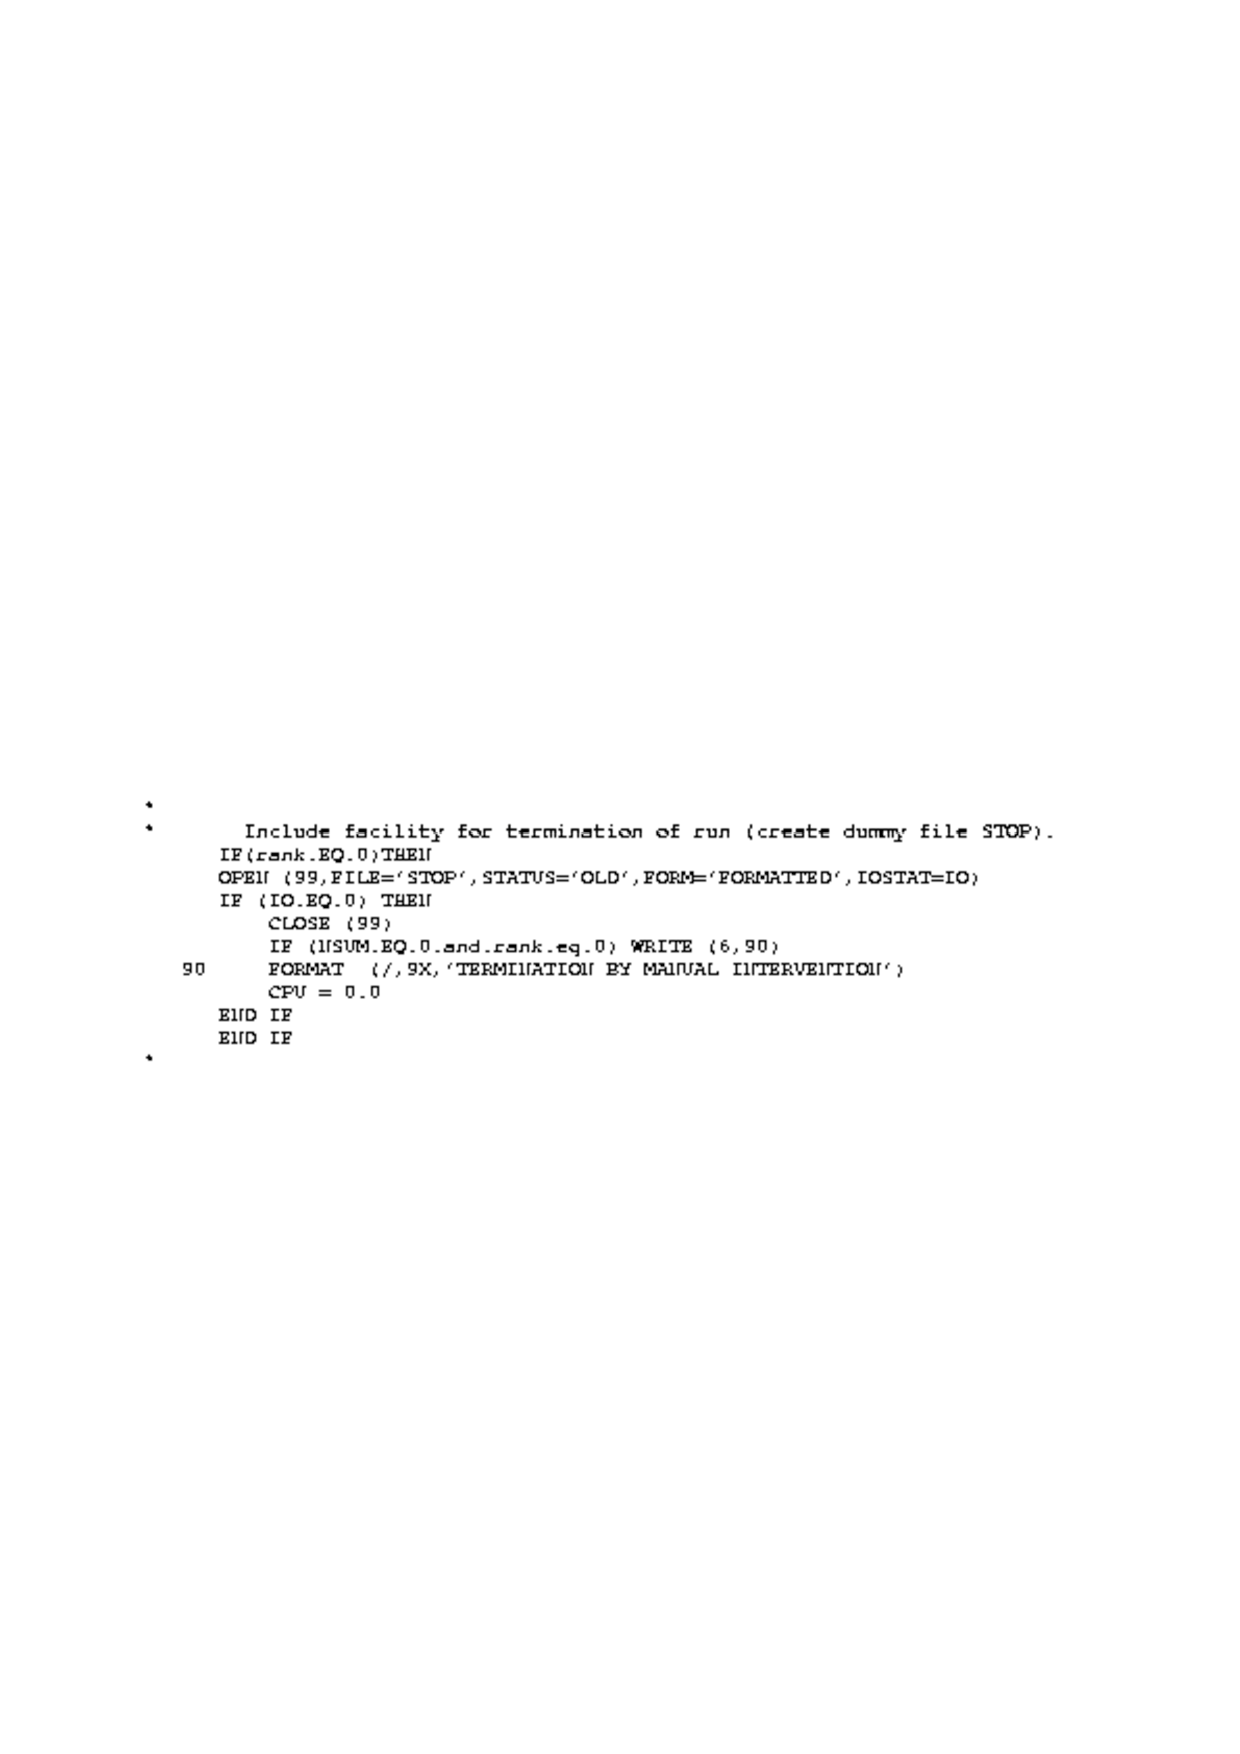
\epsfig{figure=fintgrF_p13.pdf,width=\textwidth}
  }
  \caption{Soft interruption of a simulation run in {\tt intgr.F}:
           If the dummy file ``STOP'' exists, then the run terminates.}
  \label{fig:integrF}
\end{figure}
%
The program writes out the current variables, saves a complete common
dump in {\tt comm.2\_*} and terminates.
The run can be restarted and continued from the same point where it
was left.

Before a restart, it is recommendable to copy or rename the files,
otherwise they may be overwritten.
Any file {\tt comm.2\_*} is restart-able.
The different names are just for getting common dumps at different
time units.
For example, if an irregular termination takes place, {\tt comm.2}
contains the data at some earlier time point, while {\tt comm.1}
always contains the last time data.

To restart a run, a different very short input control data file
needs to be used, because most of the control data are already
stored in {\tt comm.2\_*}~. \ff{The user should rename the desired {\tt comm.2\_*} file into {\tt comm.1}}
Only the first line corresponds to the standard input file,
but the first input variable, {\tt KSTART}, has to be changed
to ``2'' or higher.
In this case, the routine {\tt modify.F} will be entered.
%
\begin{center}
\begin{tabular}{|cp{10cm}|} \hline
{\bf KSTART} &  {\bf Function} \\  \hline
1      &  new run, start from initial values given in {\tt data.F}\\ \hline
2      &  continuation of a run without changes. With new NAMELIST input file style you can change any parameter, except for the position and velocity of the cluster in the galaxy RG(1:3) and VG(1:3), which should be calculated continuously. \\ \hline

\end{tabular}
\end{center}
%

The details of input and restart are discussed in Ch.~\ref{ch:inputvar}.

